%===============================================================================
% LaTeX sjabloon voor de bachelorproef toegepaste informatica aan HOGENT
% Meer info op https://github.com/HoGentTIN/bachproef-latex-sjabloon 
%===============================================================================

\documentclass{bachproef-tin}

\usepackage{hogent-thesis-titlepage} % Titelpagina conform aan HOGENT huisstijl
\usepackage{braket}
\usepackage{hyperref}
\usepackage{epigraph}
\usepackage{listings}
\usepackage{multirow}

%%---------- Documenteigenschappen ---------------------------------------------
% TODO: Vul dit aan met je eigen info:

% De titel van het rapport/bachelorproef
\title{The effect of quantum computing on the industry}

% Je eigen naam
\author{Jochen Dewachter}

% De naam van je promotor (lector van de opleiding)
\promotor{Antonia Pierreux}

% De naam van je co-promotor. Als je promotor ook je opdrachtgever is en je
% dus ook inhoudelijk begeleidt (en enkel dan!), mag je dit leeg laten.
\copromotor{Robbe Coudenys}

% Indien je bachelorproef in opdracht van/in samenwerking met een bedrijf of
% externe organisatie geschreven is, geef je hier de naam. Zoniet laat je dit
% zoals het is.
\instelling{---}

% Academiejaar
\academiejaar{2020-2021}

% Examenperiode
%  - 1e semester = 1e examenperiode => 1
%  - 2e semester = 2e examenperiode => 2
%  - tweede zit  = 3e examenperiode => 3
\examenperiode{2}

%===============================================================================
% Inhoud document
%===============================================================================

\begin{document}

%---------- Taalselectie -------------------------------------------------------
% Als je je bachelorproef in het Engels schrijft, haal dan onderstaande regel
% uit commentaar. Let op: de tekst op de voorkaft blijft in het Nederlands, en
% dat is ook de bedoeling!

\selectlanguage{english}

%---------- Titelblad ----------------------------------------------------------
\inserttitlepage

%---------- Samenvatting, voorwoord --------------------------------------------
\usechapterimagefalse
%%=============================================================================
%% Voorwoord
%%=============================================================================

\chapter*{\IfLanguageName{dutch}{Woord vooraf}{Preface}}
\label{ch:voorwoord}

%% TODO:
%% Het voorwoord is het enige deel van de bachelorproef waar je vanuit je
%% eigen standpunt (``ik-vorm'') mag schrijven. Je kan hier bv. motiveren
%% waarom jij het onderwerp wil bespreken.
%% Vergeet ook niet te bedanken wie je geholpen/gesteund/... heeft

This thesis was written to complete my studies in applied informatics. 
Eventhough I did not have any knowledge of quantum computing I found it really interesting and wanted to know if quantum computing could have real benefits outside the research domain.
After doing the study I found out that businesses could really gain from it. But, at this moment the technology is not developped enough to have real advantages.
This also made me realised i might want to go further in this discipline and make a career in it. Because i do think that with some more advanced research this could change the world.


This would not have been possible without the help of others.
I would like to thank Antonia Pierreux and Robbe Coudenys, they helped me with the stucture and the proofreading of this paper.
Then i would like to thank Cathy Lecoutre for proofreading this thesis.
I would like to thank Florian Unseld and Pablo Cova Fariña for giving me insights and recommendations on books to read about this topic.
Lastly i would like to thank my girlfriend, friends and parents to support me throughout my studies, it would not have been possible without them.

%%=============================================================================
%% Samenvatting
%%=============================================================================

% TODO: De "abstract" of samenvatting is een kernachtige (~ 1 blz. voor een
% thesis) synthese van het document.
%
% Deze aspecten moeten zeker aan bod komen:
% - Context: waarom is dit werk belangrijk?
% - Nood: waarom moest dit onderzocht worden?
% - Taak: wat heb je precies gedaan?
% - Object: wat staat in dit document geschreven?
% - Resultaat: wat was het resultaat?
% - Conclusie: wat is/zijn de belangrijkste conclusie(s)?
% - Perspectief: blijven er nog vragen open die in de toekomst nog kunnen
%    onderzocht worden? Wat is een mogelijk vervolg voor jouw onderzoek?
%
% LET OP! Een samenvatting is GEEN voorwoord!

%%---------- Nederlandse samenvatting -----------------------------------------
%
% TODO: Als je je bachelorproef in het Engels schrijft, moet je eerst een
% Nederlandse samenvatting invoegen. Haal daarvoor onderstaande code uit
% commentaar.
% Wie zijn bachelorproef in het Nederlands schrijft, kan dit negeren, de inhoud
% wordt niet in het document ingevoegd.

\IfLanguageName{english}{
\selectlanguage{dutch}
\chapter*{Samenvatting}

Quantum computing staat op het punt van de volgende grote ingrijpende technologie te worden.
Toch zijn het vooral de mensen die met quantum computers bezig zijn, die weten welke belangrijke rol het kan spelen in de toekomst.
Dit is de reden van het schrijven van deze studie: kennis geven over quantum computing en zijn voordelen aan het grotere publiek.
Deze studie moet de voordelen die quantum computing kan hebben uitleggen. Zo moet het CEO's en CIO's helpen met het begrijpen hoe een quantum computer werkt zodat zij de voordelen voor hun bedrijf kunnen zien.
Om te starten legt deze studie de basisbegrippen uit van quantum computers. Met de kennis rond quantum computers kan er gekeken worden naar algoritmes die beter zijn op een quantum computer dan op een klassieke computer.
Het algoritme dat onderzocht werd is Shor's algoritme. Dit is de quantum tegenhanger van de getallenlichamenzeef. Beide zijn algoritmes die grote nummers (N > $10^{100}$) gaan ontbinden in factoren.
Wat hieruit bleek is dat het aantal cijfers in het nummer een grote impact had op het klassieke algoritme. Een toevoeging van slechts 20 cijfers in het nummer kan de execution tijd doen oplopen van een klein uur tot wel 13 uur.
Shor's algoritme werkt momenteel enkel op kleine cijfers (het grootste dat een resultaat gaf was 119) en de zeef werkte enkel op grootte cijfers (N > $10^{60}$), toch kan er geconcludeerd worden uit de tijd en geheugen complexiteiten, dat een quantum algoritme de tijd en het geheugen dat nodig is voor het bekomen van een oplossing, kan verbeteren.
Momenteel staat de technologie van quantum computing nog niet ver genoeg om gebruikt te worden in gewone bedrijven, zoals bleek uit het quantum gedeelte van de studie.
De hamvraag blijft dan: hoelang zal het duren voor deze technologie wel implementeerbaar is in bedrijven?
\selectlanguage{english}
}{}

%%---------- Samenvatting -----------------------------------------------------
% De samenvatting in de hoofdtaal van het document

\chapter*{\IfLanguageName{dutch}{Samenvatting}{Abstract}}

Quantum computing is on the verge of becoming the next big thing. Yet mostly only people who work with quantum computers know what they can bring to the table.
This study should help understanding their advantages.
Its purpose is to educate CEOs and CIOs about quantum computing so that when quantum computing starts getting integrated into the businesses, they have an understanding of what it can mean for them.
The study looked into the effects that quantum computing could have on the industry and looked into its implementations in different fields.
The effects were measured by comparing two algorithms with the same task, factoring a large number (N > $10^{100}$). One of them, the number field sieve, running on a classical computer and the other, Shor's algorithm, on a quantum computer.
Even though Shor's algorithm only worked on small numbers (the highest number taht gave results was 119) and that NFS only worked on large numbers (N > $10^{60}$), there can be concluded that a quantum solution for a problem can both improve the time and the space (this is the memory) needed to find an outcome.
But at this moment quantum computers are not sophisticated enough to handle big tasks. As seen in the study, Shor's algorithm could only factor rather small numbers. Since these numbers are not used in applications today, Shor won't have any effect.
The biggest question there still is: how long will it take to improves this technology so that is has an impact on the industry?


%---------- Inhoudstafel -------------------------------------------------------
\pagestyle{empty} % Geen hoofding
\tableofcontents  % Voeg de inhoudstafel toe
\cleardoublepage  % Zorg dat volgende hoofstuk op een oneven pagina begint
\pagestyle{fancy} % Zet hoofding opnieuw aan

%---------- Lijst figuren, afkortingen, ... ------------------------------------

% Indien gewenst kan je hier een lijst van figuren/tabellen opgeven. Geef in
% dat geval je figuren/tabellen altijd een korte beschrijving:
%
%  \caption[korte beschrijving]{uitgebreide beschrijving}
%
% De korte beschrijving wordt gebruikt voor deze lijst, de uitgebreide staat bij
% de figuur of tabel zelf.

\listoffigures
\listoftables

% Als je een lijst van afkortingen of termen wil toevoegen, dan hoort die
% hier thuis. Gebruik bijvoorbeeld de ``glossaries'' package.
% https://www.overleaf.com/learn/latex/Glossaries

%---------- Kern ---------------------------------------------------------------

% De eerste hoofdstukken van een bachelorproef zijn meestal een inleiding op
% het onderwerp, literatuurstudie en verantwoording methodologie.
% Aarzel niet om een meer beschrijvende titel aan deze hoofstukken te geven of
% om bijvoorbeeld de inleiding en/of stand van zaken over meerdere hoofdstukken
% te verspreiden!

%%=============================================================================
%% Inleiding
%%=============================================================================

\chapter{\IfLanguageName{dutch}{Inleiding}{Introduction}}
\label{ch:inleiding}

De inleiding moet de lezer net genoeg informatie verschaffen om het onderwerp te begrijpen en in te zien waarom de onderzoeksvraag de moeite waard is om te onderzoeken. In de inleiding ga je literatuurverwijzingen beperken, zodat de tekst vlot leesbaar blijft. Je kan de inleiding verder onderverdelen in secties als dit de tekst verduidelijkt. Zaken die aan bod kunnen komen in de inleiding~\autocite{Pollefliet2011}:

\begin{itemize}
  \item context, achtergrond
  \item afbakenen van het onderwerp
  \item verantwoording van het onderwerp, methodologie
  \item probleemstelling
  \item onderzoeksdoelstelling
  \item onderzoeksvraag
  \item \ldots
\end{itemize}

\section{\IfLanguageName{dutch}{Probleemstelling}{Problem Statement}}
\label{sec:probleemstelling}

Uit je probleemstelling moet duidelijk zijn dat je onderzoek een meerwaarde heeft voor een concrete doelgroep. De doelgroep moet goed gedefinieerd en afgelijnd zijn. Doelgroepen als ``bedrijven,'' ``KMO's,'' systeembeheerders, enz.~zijn nog te vaag. Als je een lijstje kan maken van de personen/organisaties die een meerwaarde zullen vinden in deze bachelorproef (dit is eigenlijk je steekproefkader), dan is dat een indicatie dat de doelgroep goed gedefinieerd is. Dit kan een enkel bedrijf zijn of zelfs één persoon (je co-promotor/opdrachtgever).

\section{\IfLanguageName{dutch}{Onderzoeksvraag}{Research question}}
\label{sec:onderzoeksvraag}

Wees zo concreet mogelijk bij het formuleren van je onderzoeksvraag. Een onderzoeksvraag is trouwens iets waar nog niemand op dit moment een antwoord heeft (voor zover je kan nagaan). Het opzoeken van bestaande informatie (bv. ``welke tools bestaan er voor deze toepassing?'') is dus geen onderzoeksvraag. Je kan de onderzoeksvraag verder specifiëren in deelvragen. Bv.~als je onderzoek gaat over performantiemetingen, dan 

\section{\IfLanguageName{dutch}{Onderzoeksdoelstelling}{Research objective}}
\label{sec:onderzoeksdoelstelling}

Wat is het beoogde resultaat van je bachelorproef? Wat zijn de criteria voor succes? Beschrijf die zo concreet mogelijk. Gaat het bv. om een proof-of-concept, een prototype, een verslag met aanbevelingen, een vergelijkende studie, enz.

\section{\IfLanguageName{dutch}{Opzet van deze bachelorproef}{Structure of this bachelor thesis}}
\label{sec:opzet-bachelorproef}

% Het is gebruikelijk aan het einde van de inleiding een overzicht te
% geven van de opbouw van de rest van de tekst. Deze sectie bevat al een aanzet
% die je kan aanvullen/aanpassen in functie van je eigen tekst.

De rest van deze bachelorproef is als volgt opgebouwd:

In Hoofdstuk~\ref{ch:stand-van-zaken} wordt een overzicht gegeven van de stand van zaken binnen het onderzoeksdomein, op basis van een literatuurstudie.

In Hoofdstuk~\ref{ch:methodologie} wordt de methodologie toegelicht en worden de gebruikte onderzoekstechnieken besproken om een antwoord te kunnen formuleren op de onderzoeksvragen.

% TODO: Vul hier aan voor je eigen hoofstukken, één of twee zinnen per hoofdstuk

In Hoofdstuk~\ref{ch:conclusie}, tenslotte, wordt de conclusie gegeven en een antwoord geformuleerd op de onderzoeksvragen. Daarbij wordt ook een aanzet gegeven voor toekomstig onderzoek binnen dit domein.
\chapter{\IfLanguageName{dutch}{Stand van zaken}{State of the art}}
\label{ch:stand-van-zaken}

% Tip: Begin elk hoofdstuk met een paragraaf inleiding die beschrijft hoe
% dit hoofdstuk past binnen het geheel van de bachelorproef. Geef in het
% bijzonder aan wat de link is met het vorige en volgende hoofdstuk.

% Pas na deze inleidende paragraaf komt de eerste sectiehoofding.

% Dit hoofdstuk bevat je literatuurstudie. De inhoud gaat verder op de inleiding, maar zal het onderwerp van de bachelorproef *diepgaand* uitspitten. De bedoeling is dat de lezer na lezing van dit hoofdstuk helemaal op de hoogte is van de huidige stand van zaken (state-of-the-art) in het onderzoeksdomein. Iemand die niet vertrouwd is met het onderwerp, weet nu voldoende om de rest van het verhaal te kunnen volgen, zonder dat die er nog andere informatie moet over opzoeken \autocite{Pollefliet2011}.

% Je verwijst bij elke bewering die je doet, vakterm die je introduceert, enz. naar je bronnen. In \LaTeX{} kan dat met het commando \texttt{$\backslash${textcite\{\}}} of \texttt{$\backslash${autocite\{\}}}. Als argument van het commando geef je de ``sleutel'' van een ``record'' in een bibliografische databank in het Bib\LaTeX{}-formaat (een tekstbestand). Als je expliciet naar de auteur verwijst in de zin, gebruik je \texttt{$\backslash${}textcite\{\}}.
% Soms wil je de auteur niet expliciet vernoemen, dan gebruik je \texttt{$\backslash${}autocite\{\}}. In de volgende paragraaf een voorbeeld van elk.

% \textcite{Knuth1998} schreef een van de standaardwerken over sorteer- en zoekalgoritmen. Experten zijn het erover eens dat cloud computing een interessante opportuniteit vormen, zowel voor gebruikers als voor dienstverleners op vlak van informatietechnologie~\autocite{Creeger2009}.

In order to get a grasp on how quantum computers work, basic knowledge of quantum physics is required.
The base of the operation of quantum computers mainly lies in two quantum mechanical phenomena: superposition and entanglement.
These two phenomena combined with the limit that all operations use in computing are reversible, makes a quantum computer work the way it works.
Still the computer can't do anything on its own. It needs an algorithm that tells it what to do and when to do it.
In this case a classic algorithm just won't do the trick, since they don't manipulate qubits. A higher 'level' of algorithm is needed: a quantum algorithm.

\section{Quantum mechanics} \label{quantum mechanics}
\epigraph{If you are not completely confused by quantum mechanics, you do not understand it.}{\textit{Niels Bohr}}

In this section, the fundamentals of quantum physics used in a quantum computer will be laid out.
The focus is merely on the core items. If there is a need for a deeper understanding, refer to read the papers and articles listed in the bibliography.
The following list of mathematical terms should be familiar to you if want to understand the basics of quantum computing.

\begin{itemize}
    \item linear algebra
    \item complex numbers
    \item matrices
\end{itemize}

For more information on the mathematical aspect of this study, refer to the book of \textcite{bernhardt_2019}.

\subsection{Dirac Notation} \label{Dirac}
Also known as the bra-ketnotation, a commonly used notation in quantum mechanics. The Dirac notation is used to denote vectors \autocite{Dirac_Notation2020}.
As can be read in the Microsoft\textregistered documentations on quantum computing. The notation of vectors can be really cumbersome \autocite{Microsoft_Dirac}. To make these notations easier to read and to keep them simple, is to use the Dirac notation.

Take a vector $\vec{x}$ equal to $\begin{bmatrix}
    1 & 0 
\end{bmatrix}$.
Since this is a row matrix it can easily be written in the Dirac notation as a bra: $\bra{x}$. The same can be done for column matrices, these would become kets. As an example:
vector $\vec{y}$ = $\begin{bmatrix}
    1 \\
    0
\end{bmatrix}$ can be written as the following ket $\ket{y}$.
The Dirac notation can also be used for the inner product of vectors: the product of $\vec{x}$ and $\vec{y}$ becomes the braket $\Braket{x|y}$ as can be seen on \textcite{Dirac_Notation2020} as well on \textcite{Microsoft_Dirac}.

\subsection{Superposition} \label{superposition}
Superposition is know by most people through an experiment done by a famous Austrian scientist: Erwin Schrödinger.
In this thought experiment one would take a cat and place it in a box or bunker. 
In it there is a barrel with gunpowder or poison gas which would kill the cat 50 percent of the times. So, if the experiment was done a thousand times in 500 cases the cat would have died.
Quantum physics state that as long as the box or the bunker isn't opened the cat is in a superposition: it is death as well it is alive.
When the box or bunker is opened, the state of the cat is known \autocite{Villars_1986}.
Superposition is a state where an object has the possibility of being in either one of the basic states. Only by taking a measurement on the object, its state is defined.
For a more mathematical view on superposition, the following principle is stated in the book by \textcite{Hidary_2019}:
"The linear combination of two or more state vectors is another state vector in the same Hilbert space \footnote{A hilbert space is a complex vector space with an inner product. \autocite{Griffiths2014}} and describes another state of the system."
Another commonly used example of superposition is the polarization of light. The light we see, coming from the sun or lamps, has no particular direction of polarization.
Light is in a superposition: there is a mix of vertically and horizontally polarized light. However one particular polarization can be filtered by letting the light passing through a polarization film.
This filters the light with a polarization in one particular axis parallel of that of the film, can one particular direction be seen.
A popular polarization filter is a pair of sunglasses.

\begin{figure} [h]
    \centering
    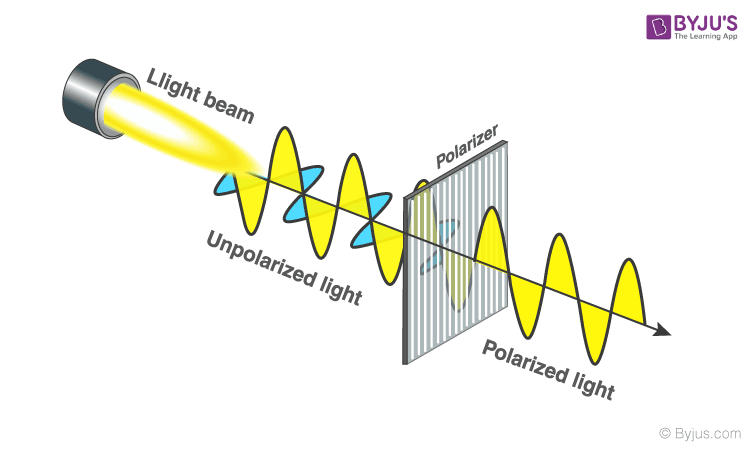
\includegraphics[width=\textwidth]{img/Polarization-of-Light-2.png}
        \caption{Polarization of light}
        \label{fig:polarization}
    \href{https://byjus.com/physics/polarization-of-light/}{Source: Byju's}

\end{figure}


\subsection{Quantum entanglement} \label{quantum entanglement}
What \textcite{Einstein} once described in a letter to Daniel M. Lipkin as "a little system of delusion of an exceedingly intelligent paranoiac concocted of incoherent elements of thought", is now a fact in the quantum mechanical world.
Quantum entanglement is the phenomenon where two or more quantum objects are coupled, they are in a state where they live together.
Or as described in in the book by \textcite{Hidary_2019}: "Two systems are in a special case of a quantum mechanical superposition called entanglement if the measurement of the one system is correlated with the state of the other system in a way that is stronger than the correlations in the classical world.".
Even though the objects are entangled, they are not physically bound to eachother. So one object could be on the north pole and the other one on the south pole.
In the paper written by Einstein, Podolsky and Rosen they describe that if one of 2 entangled particles is measured, it triggers a correlated state of the second particle \autocite{EPR}.


\section{Computing} \label{computing}
There are a lot of different types of computers: desktops, laptops, quanta and even servers are in fact just computers specialised in a specific task.
Understanding how a quantum computer works, starts at the base of that: the classical computer. Even though almost everyone uses a computer on a daily basis, not many people know how it works.


\subsection{Classical computer} \label{classical computer}
A computer consists of two main parts: software and hardware. The hardware are the physical parts that make the computer: a central processing unit (CPU), Random Access Memory (RAM) and many other parts.
Software is the term used for the programmes that run on the pc. Word, PowerPoint, ... are examples of software.

\subsubsection{Hardware} \label{hardware}
A motherboard, CPU, RAM, hard drive and a power supply are the basics every pc needs to work.
Add-ons like a Graphical processing unit (GPU or grapic card), a nice case to put everything in, a network card and cooling are nice to have and help make the pc run better or faster.
The central processing unit is the 'brain' of the computer. It makes all the calculations.
The motherboard could be seen like the 'nervous system' of the pc: everything is connected to it and allows communication between the different parts of the system.
The storage of calculations made by the CPU, is done in the RAM . Random access memory is volatile which means that when the pc is shut down everything stored on it is lost.
That is why there is a hard disk. The hard drive stores all the items that should be stored for a longer time. So when a word document is being written it starts in the RAM, but the second the file is saved it is transferred to the hard disk.
Since every component of a computer works on chips that are based on voltages, there is a need for electricity. This is where the power supply (PSU) comes in. This takes in the power from an outlet and converts it to the right amounts so the components won't get fried.
There is also hardware that is connected to the computer. This lets somebody work with it. Examples of external hardware are a monitor, keyboard and mouse, a printer, etc.
These were the basics explained so that the pc can run, but there are many other part where the info from can be found on \cite[https://edu.Fcfglobal.org/en/computerbasics/]{ComputerBasics}.

\begin{figure} [h]
    \centering
    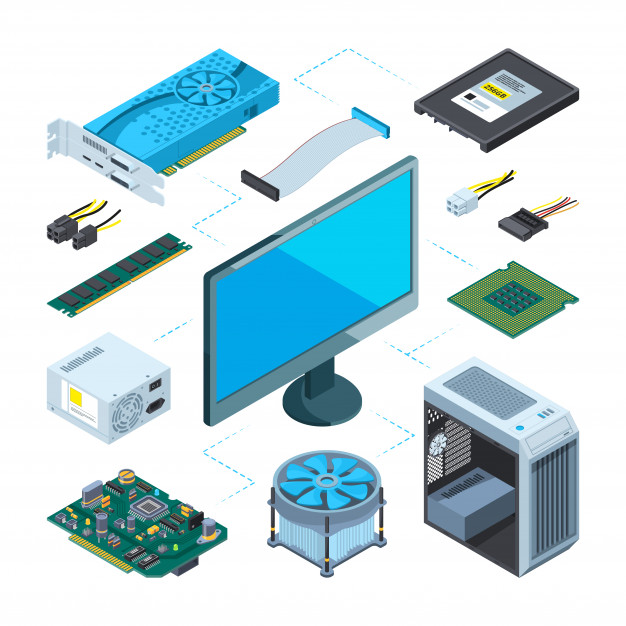
\includegraphics[width=\textwidth]{img/hardware.jpg}
        \caption{Hardware components}
        \label{fig:hardware}
        \href{https://nl.freepik.com/premium-vector/computer-hardware_4618150.htm}{Source: Freepik}
\end{figure}

The components from top to bottom and left to right: GPU, power cable, RAM, PSU, motherboard, internal cable, monitor, a fan, hard drive, data cable, CPU and the case.


\subsubsection{Software} \label{software}
Software runs on the hardware that has been described. It is an instructionlist: it tells the hardware what to do, how to do it and even when to do it \autocite{software}.
The most underlying software program is the operation system. This tells the hardware how the computer works. On top of the OS additional programs can be installed to do a variety of tasks: a text processor like word, a browser to access the internet.


\subsubsection{Operation} \label{working}
A calculation in the CPU has 3 stages: fetch, decode, execute \autocite{cpu}.
In the fetch-stage the CPU grabs an instruction from the RAM. It decodes this instruction in de decode-stage and finally when it exacly knows what the instruction means, it executes this in the execute-stage.
The CPU is made up of several billions of transistors. A tranistor is an on-off switch that, when in the 'on' state, lets current pass through.
Bits are used to represent data. This has two values: one or zero\autocite{bit}. In the case of computers this would translate to: there is a voltage detected in the transistor or there is not.
When there are two bits the calculations can start. Calculation is nothing more than taking two bits, insert those in a logical gate and the answers is spat out.
There are six logic gates: AND, OR, EXOR, NAND, NOR and EXNOR \autocite{gates}. Then there's also the inverter or the NOT-gate and a buffer, but the buffer won't be explained here.

\begin{figure} [h]
    \centering
    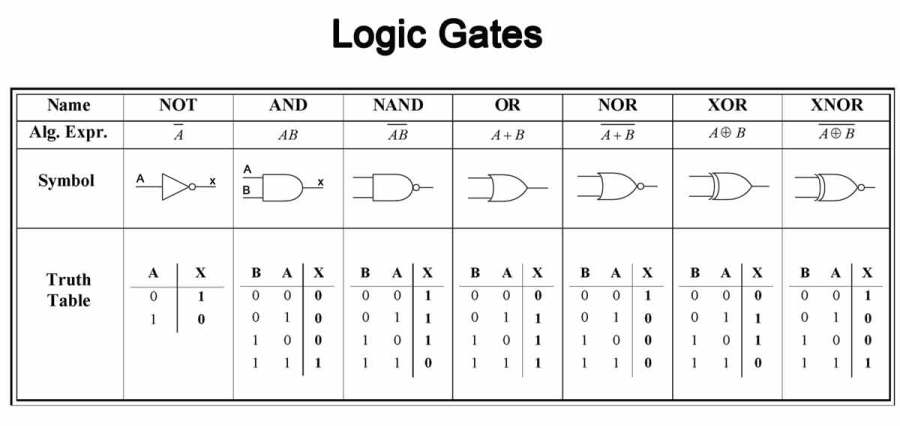
\includegraphics[width=\textwidth]{img/gates.jpg}
        \caption{Logic gates}
        \label{fig:logicGates}
        \href{https://frankcomputerscience.wordpress.com/chapter-3/}{Source: Frank Computer Science}
\end{figure}

This all means that to make faster computers, the centra processing units have to be faster. This can only be done by placing more transistors on the CPU, because more transistors means more calcuations.
The number of transistors that can be put on a chip is still rising. This is defined by \textcite{Moore1965}'s law: it started out with every year the amount doubles. But since they are getting closer to the physical boundaries, this changed to every two years.


\subsection{Quantum computer} \label{quantum computer}
The big difference between the classical computer and a quantum computer is the unit of a calculation: quantum computers don't use bits but use qubits.
The qubit allows faster calculations because of it's quantum mechanical nature.


\subsubsection{The qubit} \label{qubit}
A qubit is the analogue of the classical bit. It has 2 states: $\ket{0}$ and $\ket{1}$, but it can be in a linear combination of those 2 base states called the superposition \autocite{thequbit}.
\begin{equation}
    \ket{\phi} = \alpha * \ket{0} + \beta * \ket{1}
\end{equation}
This is the representation of a superposition, where $\alpha$ and $\beta$ are probability amplitudes(complex numbers) used to calculate the probability density.


The state of a qubit can also be represented visually by using the bloch sphere. The bloch sphere represents the pure states \footnote{A pure state of a system is a state that cannot be represented by a mixture of other states as can be seen in the proof of that theorem in \textcite{Ballentine2014}} of a 2-level quantum system on the surface of the sphere, and represents mixed states in its interiour.
There are six commonly known basic states on the bloch sphere:

\begin{itemize}
    \item On the Z-basis
        \begin{itemize}
            \item $\ket{0}$
            \item $\ket{1}$
        \end{itemize}
    \item On the X-basis
        \begin{itemize}
            \item $\ket{+} = \frac{\ket{0} + \ket{1}}{\sqrt{2}}$
            \item $\ket{-} = \frac{\ket{0} - \ket{1}}{\sqrt{2}}$
        \end{itemize}
    \item On the Y-basis
        \begin{itemize}
            \item $\ket{R} = \frac{\ket{0} + i \ket{1}}{\sqrt{2}}$
            \item $\ket{L} = \frac{\ket{0} - i \ket{1}}{\sqrt{2}}$
        \end{itemize}
\end{itemize}

Qubits can be physically implemented by many things: the polarization of photons, spin states of an atom or electron, etc \autocite{thequbit}.
As an example, let's make a qubit from the spin of an electron. It is known that the spin-state(up or down) can be changed by subjecting the electron in a magnetic field.
\textcite{Stern} found the atomic spin in their experiment in 1922. In the experiment they shot a beam of silveratoms through a magnetic field in a vacuum and 'caught' the atoms on a plate. After the experiment they looked at this plated and saw that instead of the atoms being distributed evenly on the plate, there were two big bundles.
One bundle was slightly higher than the center and the other slightly lower. Knowing that a magnetic field has an influence on atoms, can be used as an advantage. As seen in the Zeeman effect: applying an external magnetic fields ensures that the spinstate that the atom is in, is in a higher energy level(an exited state) than the other spinstate \autocite{Zeeman}.
Because atoms want to be in the lowest possible energystate(the groundstate), the atom will change its spin. 

\begin{figure} [h]
    \centering
    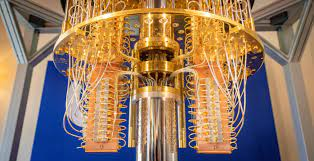
\includegraphics[width=\textwidth]{img/qcomputer.jpg}
        \caption{The cooling system of a quantum computer}
        \label{fig:Quantum computer cooling}
        \href{https://www.cnet.com/news/quantum-computing-research-helps-ibm-win-top-spot-in-patent-race/}{Source: CNET}
\end{figure}

\subsubsection{The hardware}
Since generating a qubit is very difficult work and the slightest change may give errors in calculations, there is a big need to control the outside noice.
The article by \textcite{Cooling} states that to minimize the chance of qubits flipping between quantum states, the computer has to be cooled so that the energy level inside it is at its lowest possible point.
Since a qubit heats up when it's used in calculations \autocite{Cooling}, the cooling must be excellent. This is why they cool the qubit to temperatures around the absolute zero: zero degrees Kelvin (0°K or -273,15°C).
This cooling system is what makes the quantum computer so big, most of the photo's you see online like the one seen in figure \ref{fig:Quantum computer cooling}, are in fact just the refrigerators. This is the quantum part of the quantum computer. But quantum computers don't work like conventional computers. They can not connect to the internet on their own and they can't store a lot of data on drives, etc.
This requires a classical part: a classical computer that is connected to the quantum computer so that interaction with it can be achieved. This part is used to build the applications for the quantum computer \autocite{qhardware}.

The processor itself is the central part as seen in figure \ref*{fig:Quantum computer cooling}, all the other yellow parts can be seen is the cooling system.
A quantum computer consists of 4 hardware layers: quantum data plane, control and measurement plane, control processor plane and host processor \autocite{qhardware}.

\begin{enumerate}
    \item The quantum data plane

        \quad The quantum data plane is the core of the entire computer. In this 'plane' the qubits are found.

         
    \item The control and measurement plane

        \quad The control and measurement plane is the plane where all the operations on the qubits happen. It takes the signals of the control processor plane and converts them so the operations can be executed.
        Next to converting signals to execute operations, the control and measurement plane is also in charge of converting the signals from the measurements to binary data so that the data can be processed.
        This plane holds back the speed of the computer: this can not exceed the speed to create a control signal.

    \item The control processor plane

        \quad In the control processor plane, the controlling of all the operations takes place. It determines the sequence of operations on the qubits, but it doesn't execute them. Its input is the code of a program and outputs the right instructions to the control and measurement plane.

    \item The host processor

        \quad This is a classical computer that manages the 'normal' side of the operations. The applications are build to run on the control processor. Other functions of the host are providing storage to the quantum computing and sometimes networking.

\end{enumerate}
%%=============================================================================
%% Methodologie
%%=============================================================================

\chapter{\IfLanguageName{dutch}{Methodologie}{Methodology}}
\label{ch:methodologie}

%% TODO: Hoe ben je te werk gegaan? Verdeel je onderzoek in grote fasen, en
%% licht in elke fase toe welke stappen je gevolgd hebt. Verantwoord waarom je
%% op deze manier te werk gegaan bent. Je moet kunnen aantonen dat je de best
%% mogelijke manier toegepast hebt om een antwoord te vinden op de
%% onderzoeksvraag. 

In the study two different algorithms will be used to compare quantum computing with classical computing. 
The fact that there are two algorithms and not just one is because a quantum computer can't run a normal algorithm: is has to be updated to a new form, the quantum algorithm.
This chapter will explain more about the algorithms, which one is chosen and how to rewrite it to a quantum algorithm. Since there will be a look into the complexities of an algorithm, there will be an explanation on what this is.
Both the time and space complexities will be clarified. Running the classical algorith is easy since it can be done on a classical computer. For the quantum algorithm: it has to be run on a quantum computer.
To simulate this the study will be using IBM's Quantum composer, but more information about that in \ref{sec:Composer}.
\section{Algorithms}
Originally there was a survey build for this study from which algorithms that are frequently used in businesses nowadays would come. This survey was spread out to the public across multiple media sources, and on several occasions.
Yet there was not much response on this survey, so the decision to not use this was made. Another algorithm will be used: the algorithm to find factors of large numbers. This was chosen because this is, at the moment writing, this forms the biggest 'threat' from quantum computing to the world.
This is because RSA encryption is based on the fact that factorization of large numbers, like bank numbers or cryptosystems \autocite{Shor}, takes a very long time to do for classical computers. But if a quantum computer could do it in mere seconds or even minutes the entire bankin system could fall, no transaction would be safe anymore.
This algorithm has already been made and is known as Shor's algorithm \autocite{Shor}.
\subsection{Complexities of algorithms}
\label{subsec:Complexities}
There are two complexitites used to describe algorithms: Time and Space. Those complexities describe the efficiency of the algorithm. By doing this there is a general way to compare two algorithms with eachother: calculate the complexitites of both and compare them.
Time complexity is the time needed to run an algorithm as a function of the length of the input \autocite{Timecomp}. The length of the input is the amount of operations that have to be run. Say there is an algorithm with a for-loop from 1 to 100.
In this loop it just adds the numbers up, then the algorithm has to run 100 operations inside the loop and 100 operations to check if the loop is fulfilled. That makes a total of 200 operations just to add the numbers from 1 to 100.
The amount of time needed can also differ from computer to computer: a pc with a better processor, say an Intel Core i7 with a base frequency of 4,9 GHz may have significant better times than a lower quality processor: Intel Core i3 with a base frequency of 2,9 GHz.
To note the time complexity of an algorithm, the big-O notation is used. As read in \textcite{Hidary_2019}, the big-O notation is used to describe the asymptotic upper bound or the worst case scenario. In the case of time complexity that's the logest time it will take to run the algorithm.
In the space complexity, the memory needed for to run the algorithm is taken into account to calculate the efficiency of the algorithm \autocite{Abhishek2021Ruimte}. As in time complexity, space complexity too uses the big-O notation to note it's worst case scenario. Another notation that could be used is the asymptotic lower bound or the best case scenario: the omega notation.
In this study, only the big-O notation will be handeled when speaking about the complexity of an algorithm.
\subsection{Everything about quantum algorithms}
Eventhough all the classical algorithms can be run on a quantum computer, the superpositions of qubits or entanglement would never be used \autocite{qalgo} and \autocite{quantumalgo} ans thus it would make the quantum computer a very expensive computer.
The term quantum algorithm is only used for an algorithm when it uses features of quantum computing like superposition or entanglement.
Eventhough a quantum computer may be able to solve some of the algorithms faster than a classical computer, it can not help with undecidable problems. If there is no know classical algorithm to solve a problem, there will not be a quantum one \autocite{undecidable} and \autocite{quantumalgo}.
The algorithm used in this study is an algorithm used for factoring very large numbers. The best classical algorithm to do is is known as the general number field sieve \autocite{GNFS}, and its quantum counterpart is known as Shor's algorithm \autocite{Shor}.
Quantum algorithms are often shown in a quantum circuit as can be seen in figure \ref{fig:Quantum circuit}. A quantum circuit has 2 main elements: the qubits represented by the horizontal lines and the quantum gates or operations represented by the squares on the lines.
When a qubit line crosses a gate it means that that specific gate is used on that qubit. There are different gates, but those will be explained in \ref{subsubsec:gates}.

\begin{figure} [h]
    \centering
    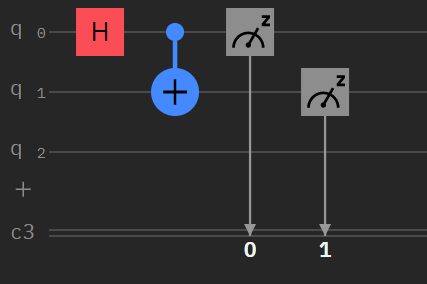
\includegraphics[width=\textwidth]{img/circuitVB.PNG}
        \caption{This is an example of a simple quantum circuit}
        \label{fig:Quantum circuit}
\end{figure}

\section{Quantum composer}
\label{sec:Composer}
Quantum composer is a tool to build quantum circuits. After building the circuits, they can be run on the quantum computer at IBM. This is an easy-to-use beginners tool. The circuits can be made by a drag and drop system.
At the same time that the circuits is being build, the tool converts it into code in OpenQuasm2.0. It also shows the probabilities of each qubit and the blockspehere representation of the qubits.
In figure \ref{fig:Quantum composer} a screenshot of Quantum composer can be seen. At the top all the gates can be found and right under the gates the circuits is build. The right part of the screen is the OpenQuasm2.0 code.
The bottom shows the blochsphere-representation and the probabilities.

\begin{figure} [h]
    \centering
    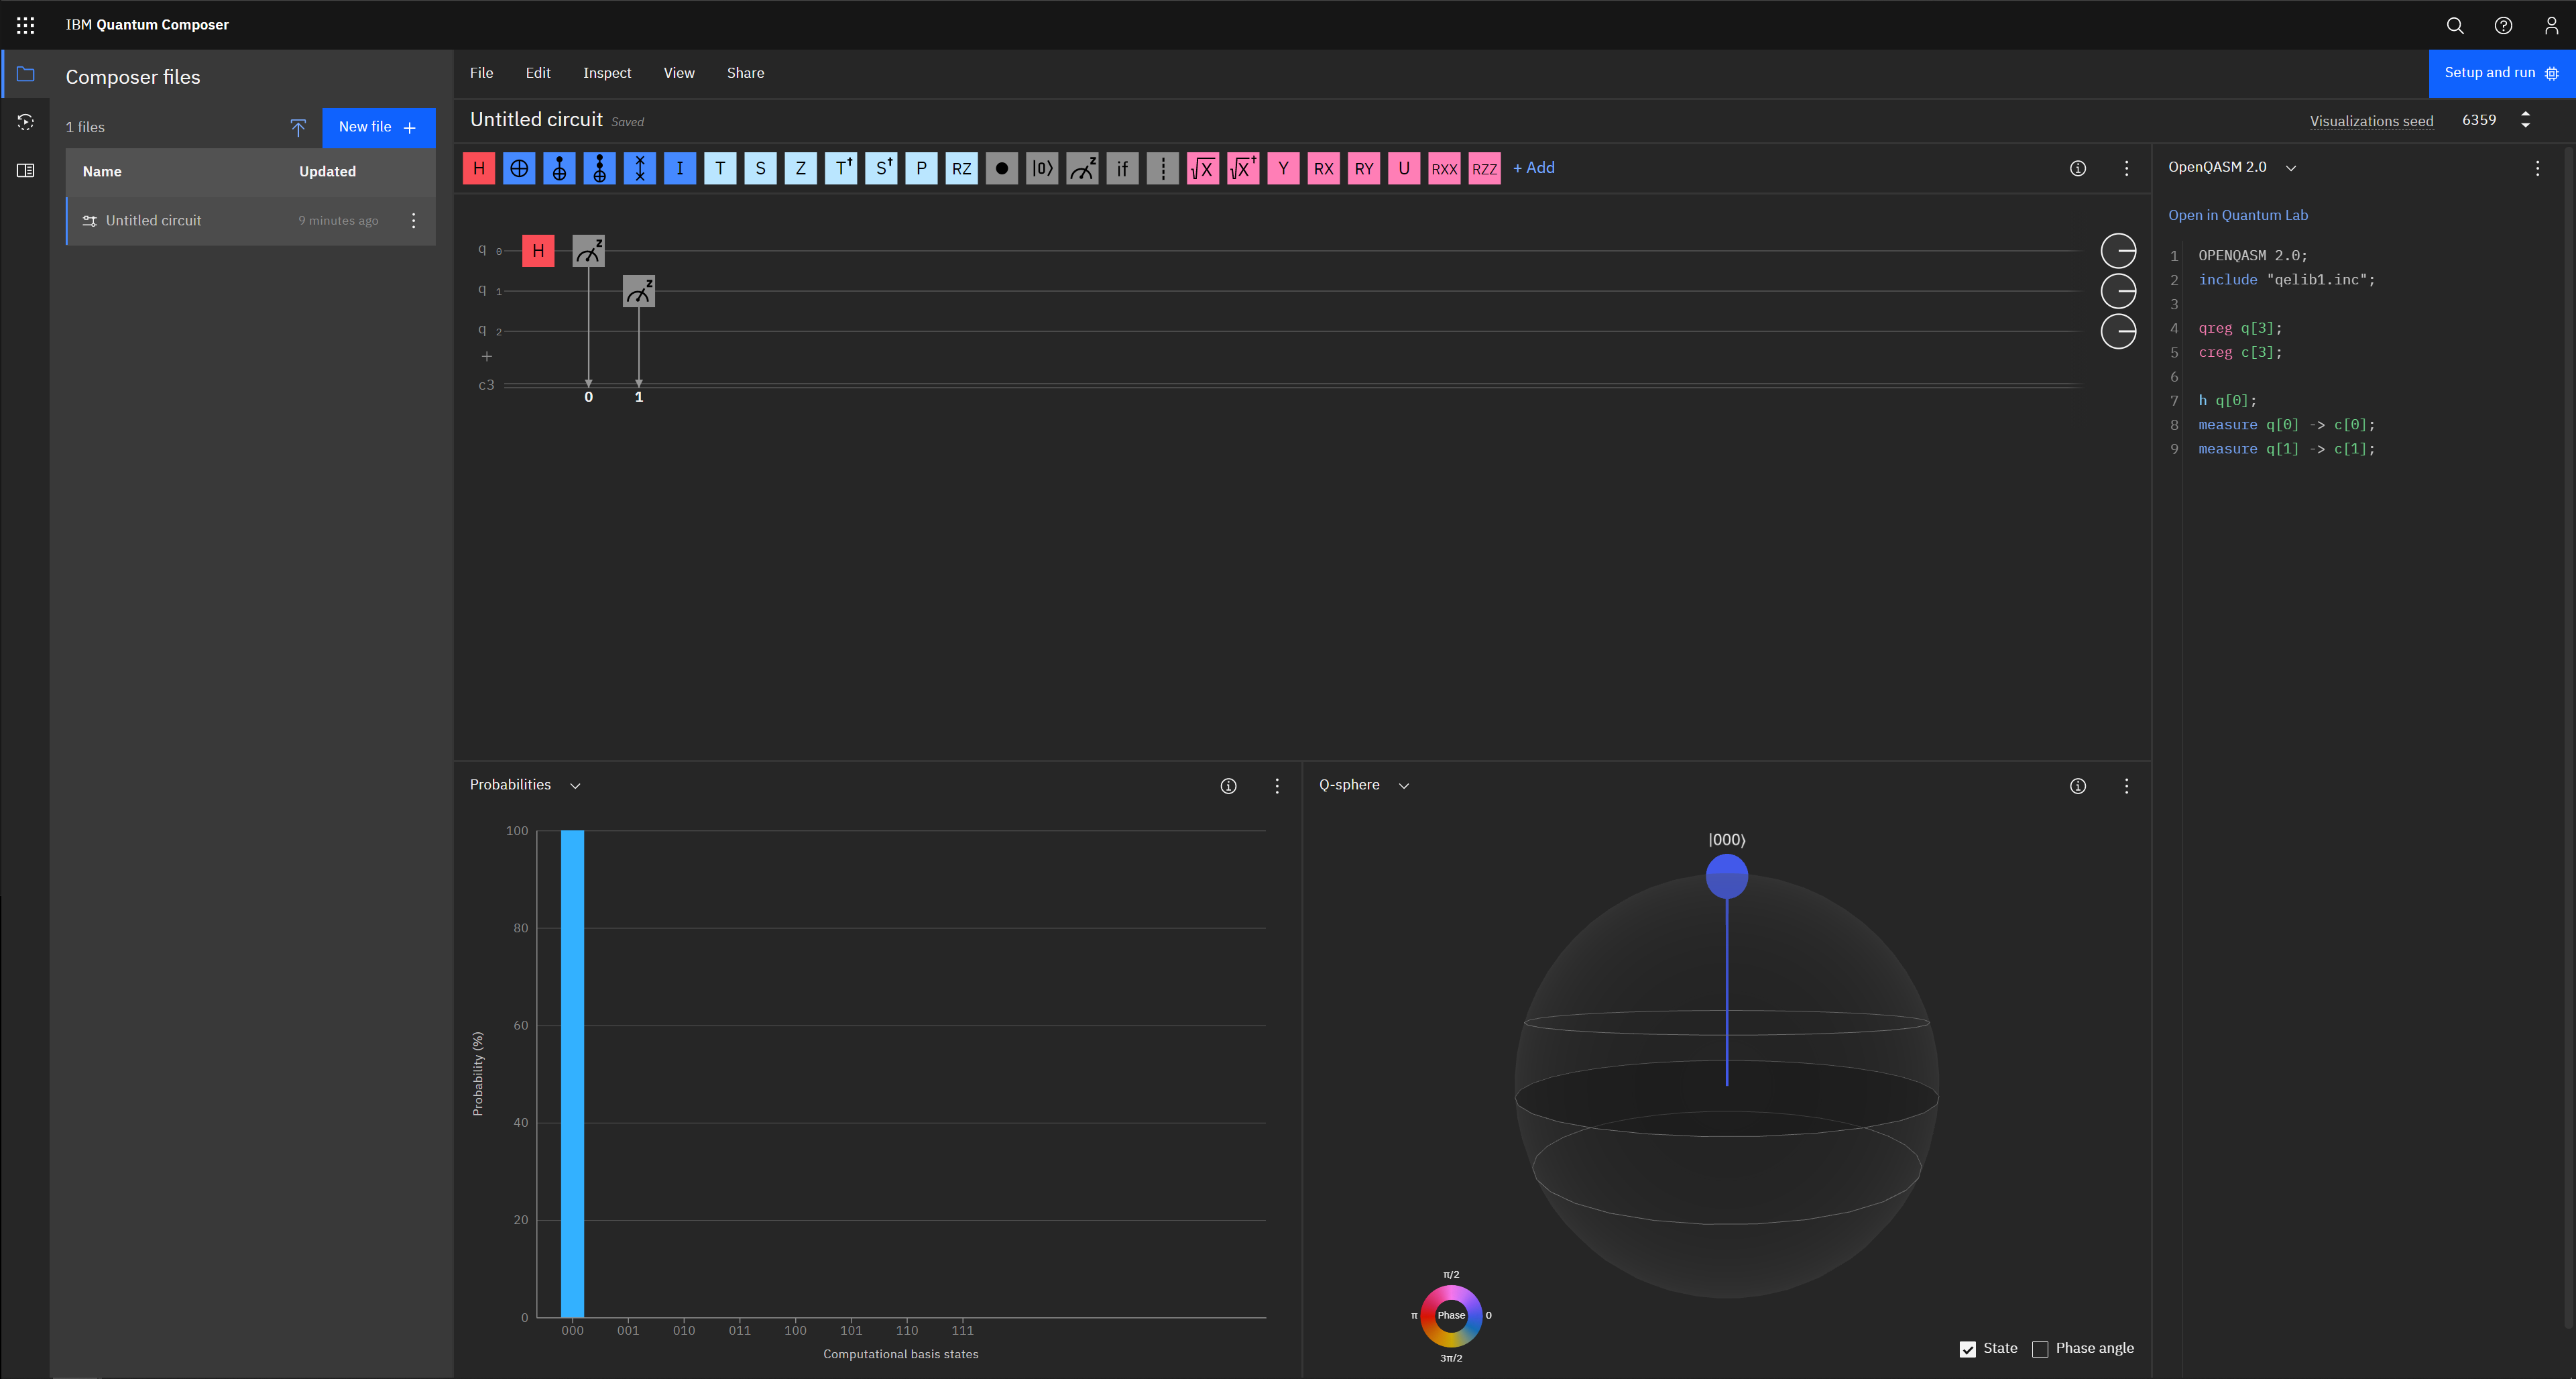
\includegraphics[width=\textwidth]{img/composer.PNG}
        \caption{Screenshot of Quantum composer}
        \label{fig:Quantum composer}
\end{figure}
%%=============================================================================
%% Onderzoek
%%=============================================================================

\chapter{\IfLanguageName{dutch}{Onderzoek}{Study}}
\label{ch:onderzoek}



In this study there will be a comparison between the GNFS algorithm on a classical computer and Shor's algorithm on a quantum computer.
Section \ref{sec:Other algorithms} will discuss some other algorithms that can show the benefits of quantum computing in the industry. To conclude there will be looked into the main industries it could be used in.

\section{The comparison}
\subsection{General Number Field Sieve}
\subsection{Shor's algorithm}
\subsubsection{Gates}
\label{subsubsec:gates}
For building circuits, this study will be using IBM's quantum composer. It can be used in two differnt ways: drag and drop or writing code.
As mentioned in section \ref{sec:Composer} writing code in the composer is done with OpenQASM2.0 and the drag and drop uses lines that represent qubits on which gates or operators can be placed.
All the gates used in the composer will be explained first. All the information of the operations can be found on the webside of IBM \footnote{$https://quantum-computing.ibm.com/composer/docs/iqx/operations_glossary$} on quantum computing as well as in \textcite{Hidary_2019} section 3.1 Quantum operators.
There are 5 types of gates: classicals, quantums, phases, non-unitaries and the Hadamard gate. Most of the gates are reversible: when the same operation is used twice on a qubit, it's state will be the same as the starting state \autocite{reversible_gates, revgates}.

The first gates that will be discussed are the classical gates, also known as Pauli gates. In this group 4 gates can be found: the NOT gate, the CNOT gate, the Toffoli gate and the SWAP gate.
In figure \ref{fig:classical gates} the representation of the classical gates in composer is given in the following order, NOT, CNOT, Toffoli and SWAP.
The not gate, or Pauli X gate, flips the state of a qubit. The controlled not gate, or CX, uses 2 qubits. One qubit is the target that will be flipped if the controll qubit is in state $\ket{1}$. It can also function as an operation to make an entanglement.
In this case if the controll qubit is in a superposition, both qubits will be entangled. The Toffoli gate acts as a double CNOT gate. It uses two controll qubits that have to be in the $\ket{1}$ state to flip the target.
Lastly there is the SWAP gate. This is self-explanatory because it just swaps the states of two qubits. There is a special gate called the identity gate. In fact it's not a gate at all, this 'gate' is a blank unit in the gate time to ensure nothing can happen with that qubit at that specic moment.

Next up are the phase gates. This group of gates exists of the T gate, S gate, Z gate, T$\dagger$ gate, S$\dagger$ gate, phase gate and the RZ gate, and are shown in figure \ref{fig:phase gates}. These gates shift the phase of the qubits.
The T$\dagger$ and S$\dagger$ gates are the inverse gates of the respectively T and S gate. And the T, S and Z gate are just 'special' cases of the phase gate.
In table \ref{tab:pgates} the matrix representation of each gate can be found.

There are 5 different non-unitary operators or modifiers. These operators are reset, measurement, the control modifier, IF and the barrier operation as shown in figure \ref{fig:non-uni gates}.
The reset operations resets the qubit to the $\ket{0}$ state. This operation doesn't take any previous state into consideration and is not reversible.
The measurement operation also is not reversible and measures the qubit. So it's output gives the value of the qubit in the standard basis.
Applying an IF operation can give conditions to quantum gates. The conditions in the if operations depend on the state of the classical register, not the quantum one.
When a circuit is executed the computer will try to combine gates to increase the efficiency. If these combinations should not happen, de barrier operation can be used.
Lastly the control modifier is used with another operation. Say for example the Z-gate is used and a control modifier is applied to that, the Z-gate will only be executed if the qubit on which the control lays is in state $\ket{1}$.

The Hadamard gate is used to make superpositions. When applying this gate to a qubit in state $\ket{1}$ or $\ket{0}$, it rotates it resulting respective states $\ket{-}$ and $\ket{+S}$

$\sqrt{X}$, $\sqrt{X}$$\dagger$, Y, RX, RY, RXX, RZZ and U make up the last set of gates: the quantum gates. 
The RX and RY respectively rotate the qubit around the x- and y-axis. The Y-gate is a special case of RY, where $\theta$ equals $\pi$.
With the U-gate any single-qubit gate can be made. This is because it takes 3 angles as an input.
$\sqrt{X}$ and it's inverse $\sqrt{X}$$\dagger$ can make a superposition if the qubit it is qpplied to is in state $\ket{0}$. If the gates is applied twice in a row the output wil give a standard NOT-gate.
In table \ref{tab:qgates} a representation can be found on the matrixes of every quantum gate.

\begin{figure} [h]
    \centering
    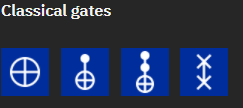
\includegraphics[width=\textwidth]{img/classical-gates.PNG}
        \caption{A visual representation of the classical gates}
        \label{fig:classical gates}
\end{figure}

\begin{table}[]
\label{tab:pgates}
        \begin{tabular}{l|l}
        \hline
        \multicolumn{1}{|l|}{Phase Gate}  & \multicolumn{1}{l|}{Matrix representation of the gate}               \\ \hline
        T                                 & $\begin{pmatrix}1&0 \\ 0& \exp(i\frac{\theta}{4})\end{pmatrix}$      \\
        Z                                 & $\begin{pmatrix}1&0 \\ 0& -1\end{pmatrix}$                           \\
        S                                 & $\begin{pmatrix}1&0 \\ 0& i\end{pmatrix}$                            \\
        T$\dagger$                        & $\begin{pmatrix}1&0 \\ 0& \exp(-i\frac{\theta}{4})\end{pmatrix}$     \\
        S$\dagger $                       & $\begin{pmatrix}1&0 \\ 0& -i\end{pmatrix}$                           \\
        P                                 & $\begin{pmatrix}1&0 \\ 0& \exp(i\lambda)\end{pmatrix}$               \\
        RZ                                & $\begin{pmatrix}\exp(-i\frac{\lambda}{2})&0 \\ 0& \exp(i\frac{\lambda}{2})\end{pmatrix}$                                    
        \end{tabular}
        \caption{Matrix representations of the phase gates.}
\end{table}
    
\begin{figure} [h]
    \centering
    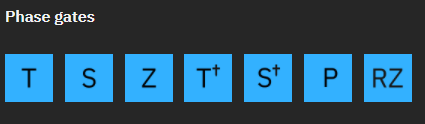
\includegraphics[width=\textwidth]{img/phase-gates.PNG}
        \caption{A visual representation of the phase gates}
        \label{fig:phase gates}
\end{figure}

\begin{figure} [h]
    \centering
    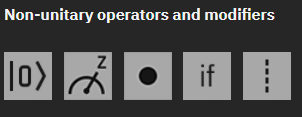
\includegraphics[width=\textwidth]{img/non-unitary-gates.PNG}
        \caption{A visual representation of the non-unitary gates}
        \label{fig:non-uni gates}
\end{figure}

\begin{figure} [h]
    \centering
    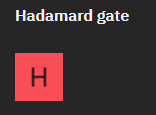
\includegraphics[width=\textwidth]{img/hadamard-gate.PNG}
        \caption{A visual representation of the hadamard gate}
        \label{fig:hadamard gates}
\end{figure}

\begin{table}[]
\label{tab:qgates}
        \begin{tabular}{l|l}
        \hline
        \multicolumn{1}{|l|}{Phase Gate}  & \multicolumn{1}{l|}{Matrix representation of the gate}                                                                                                                                                                                                                         \\ \hline
        RX                                & $\begin{pmatrix} \cos\frac{\theta}{2}&-i\sin\frac{\theta}{2}              \\ -i\sin\frac{\theta}{2}&\cos\frac{\theta}{2}                                                                                                                                        \end{pmatrix}$ \\
        RY                                & $\begin{pmatrix} \cos\frac{\theta}{2}&-\sin\frac{\theta}{2}               \\ \cos\frac{\theta}{2}&\sin\frac{\theta}{2}                                                                                                                                          \end{pmatrix}$ \\
        RXX                               & $\begin{pmatrix} \cos\frac{\theta}{2}&0&0&-i\sin\frac{\theta}{2}          \\ 0&\cos\frac{\theta}{2}&-i\sin\frac{\theta}{2}&0                           \\ 0&-i\sin\frac{\theta}{2}&\cos\frac{\theta}{2}&0 \\ -i\sin\frac{\theta}{2}&0&0&\cos\frac{\theta}{2}    \end{pmatrix}$ \\                               
        RZZ                               & $\begin{pmatrix} \exp(-i\frac{\theta}{2})&0&0&0                           \\ 0&\exp(i\frac{\theta}{2})&0&0                                             \\ 0&0&\exp(i\frac{\theta}{2})&0 \\ 0&0&0&\exp(-i\frac{\theta}{2})                                       \end{pmatrix}$ \\         
        $\sqrt{X}$                        & $\begin{pmatrix} 1+i&1-i                                                  \\ 1-i&1+i                                                                                                                                                                            \end{pmatrix}$ \\
        $\sqrt{X}\dagger$                 & $\begin{pmatrix} 1-i&1+i                                                  \\ 1+i&1-i                                                                                                                                                                            \end{pmatrix}$ \\
        U                                 & $\begin{pmatrix} \cos\frac{\theta}{2}&-\exp(i\lambda)\sin\frac{\theta}{2} \\ \exp(i\phi)\sin\frac{\theta}{2}&\exp(i(\phi+\lambda))\cos\frac{\theta}{@}                                                                                                          \end{pmatrix}$ \\
        Y                                 & $\begin{pmatrix} 0&-i \\ i&0                                                                                                                                                                                                                                    \end{pmatrix}$                                   
        \end{tabular}
        \caption{Matrix representations of the quantum gates.}
\end{table}

\begin{figure} [h]
    \centering
    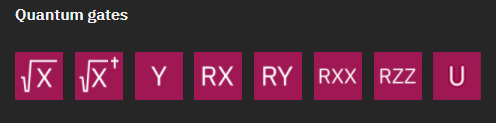
\includegraphics[width=\textwidth]{img/quantum-gates.PNG}
        \caption{A visual representation of the quantum gates}
        \label{fig:quantum gates}
\end{figure}

\subsubsection{The algorithm}
\section{Other algorithms}
\label{sec:Other algorithms}
\section{The use of quantum computing}

% Voeg hier je eigen hoofdstukken toe die de ``corpus'' van je bachelorproef
% vormen. De structuur en titels hangen af van je eigen onderzoek. Je kan bv.
% elke fase in je onderzoek in een apart hoofdstuk bespreken.

%\input{...}
%\input{...}
%...

%%=============================================================================
%% Conclusie
%%=============================================================================

\chapter{Conclusie}
\label{ch:conclusie}

% TODO: Trek een duidelijke conclusie, in de vorm van een antwoord op de
% onderzoeksvra(a)g(en). Wat was jouw bijdrage aan het onderzoeksdomein en
% hoe biedt dit meerwaarde aan het vakgebied/doelgroep? 
% Reflecteer kritisch over het resultaat. In Engelse teksten wordt deze sectie
% ``Discussion'' genoemd. Had je deze uitkomst verwacht? Zijn er zaken die nog
% niet duidelijk zijn?
% Heeft het onderzoek geleid tot nieuwe vragen die uitnodigen tot verder 
%onderzoek?

This study tried to find an answer on what the effect of quantum computing could be on the industry.

To start a comparison between classic and quantum computing was done. This came to the conclusion that by using quantum mechanics significant improvements could be reached.
The time and space complexities both could be lowered, which can help in solving problems that could not be solved before in a meaningful time frame.
As can be seen the effect of the input data in an algorithm can drasticly change the runtime of it. For example, adding only 20 digits to a number to factor can change the runtime from a little bit under an hour to 13 hours.
And eventhough it's not visible from the experiment itself, this does not happens as extreme on a quantum computer as on a classical one.

At the momement of writing the industries that could benefit most of quantum computing are the fields where research is done. The technology itself is to expensive and not advanced enough to start using in businesscompanies.
When the more advanced quantum computers are made, other industries, like financial institutions, chemistry companies and such can also benifit from this.



%%=============================================================================
%% Bijlagen
%%=============================================================================

\appendix
\renewcommand{\chaptername}{Appendix}

%%---------- Onderzoeksvoorstel -----------------------------------------------

\chapter{Onderzoeksvoorstel}

Het onderwerp van deze bachelorproef is gebaseerd op een onderzoeksvoorstel dat vooraf werd beoordeeld door de promotor. Dat voorstel is opgenomen in deze bijlage.

% Verwijzing naar het bestand met de inhoud van het onderzoeksvoorstel
%---------- Inleiding ---------------------------------------------------------

\section{Introductie} % The \section*{} command stops section numbering
\label{sec:introductie}

In dit onderzoek wordt de impact onderzocht van quantumcomputers op de industrie.
Op dit moment bestaan er 3 soorten computers: de klassieke computer, supercomputers en de quantumcomputer.
De klassieke computer kent iedereen en een supercomputer is hier eigenlijk een veel betere variant van: deze hebben meer rekenkracht, maar de principes blijven hetzelfde.
Nu zijn er nog steeds problemen die we niet efficient kunnen oplossen met onze computers.
Voorbeelden hiervan zijn: simulaties van molecules en quantumfysische begrippen, RSA (hèt encryptiealgoritme dat in transacties gebruikt wordt), zoeken in databanken(deze databanken hebben miljoenen entries), enz.
Het probleem zit niet bij de kracht van de tegenwoordige computers, maar in de tijd die een klassieke computer nodig heeft om een proces uit te voeren.
Dit komt omdat een klassieke computer alles 1 voor 1 moeten overlopen en verwerken en hierbij kunnen quantumcomputers van pas komen.

%---------- Stand van zaken ---------------------------------------------------

\section{State-of-the-art}
\label{sec:state-of-the-art}

Een klassieke computer werkt met bits: een 0 of een 1. In een computer wordt een bit gemaakt door een transistor.
Dit is eigenlijk gewoon een kleine schakelaar waar elektriciteit door gaat.
De transistor kan dan open staan en het signaal door laten (een één) of toe zijn en het signaal tegen houden (een nul).
Door middel van verschillende transistoren aan elkaar te koppelen onstaat een chip en kunnen er complexe bewerkingen uitgevoerd worden.
De transistor is dus de belangrijkste bouwsteen van de hedendaagse computer. Hoe beter de computer moet zijn, hoe beter de chip ofwel hoe meer transistoren.
Ieder jaar worden onze chips beter, maar niet groter. Het is zelfs zo dat volgens de Wet van \textcite{Moore1965} iedere 2 jaar het aantal transistoren verdubbeld wordt op een chip.
Nu kan dit enkel zo zijn doordat onze transistoren kleiner worden door de steeds verbeterende technologie en dit is inderdaad zo, de transistor is van enkele centimeters groot gekrompen naar enkele nanomters groot.
Maar dit kan niet blijven doorgaan. Zo is er berekend geweest dat de Wet van \textcite{Moore1965} nog tot rond 2036 zou gelden\autocite{Powell2008}.  Momenteel is een transistor zodanig klein dat als men nog veel kleiner zou gaan, een elektron (een negatief geladen deeltje waardoor electriciteit kan werken) door de transistor door kan gaan.
Het laatstgenoemde effect wordt ook wel het Tunneleffect genoemd. Normaal gezien kan een electron niet door de potentiaalbarricade van een transistor, maar door het golfgedrag van een electron bestaat er een kleine kans dat dit wel gebeurt als de transistor klein genoeg is zoals te zien in figuur 1.

In quantumcomputers spreekt men niet meer van een bit maar van een quantumbit of qubit. Dit kan door een paar dingen voorgesteld worden, maar er wordt vaak gekozen voor een foton (een lichtdeeltje) of een elektron. 
Net zoals het normale bit kan dit in 2 staten zijn: nul of één. Maar er is nog een derde staat mogelijk, namelijk een superpositie van de 2.
In deze superpositie is het bit zowel een nul als een één. De kans dat een qubit een één of een nul wordt hangt af van de quantum staat die vooraf ging aan de meting.
Vanop het moment dat het bit gemeten wordt, dus dat men kijkt wat de waarde van het bit is, valt deze superpositie weg en ligt de waarde van het bit vast.
Het is net door deze superpositie van beide staten dat een quantumcomputer zoveel sneller werkt.
Een laatse fenomeen dat te vinden is bij quantumcomputers is entanglement. Dit verschijnsel 'hangt' 2 of meer deeltjes aan elkaar vast zoals beschreven in \textcite{Bengtsson2017}.
Zo kan men het ene deeltje niet beschrijven zonder het andere te vernoemen. Als het ene deeltje een 1 waarde aanneemt tijdens de meting is men er zeker van dat het andere deeltje een nul-waarde aanneemt bij eenzelfde meeting.

Het zijn net deze 3 quantumfenomenen die ervoor zorgen dat een quantumcomputer werkt. Het is wel echter zo dat een quantumcomputer geen klassieke computer kan vervangen.
Quantumcomputers kunnen enkel in bepaalde contexten gebruikt worden, de aparte stappen om een algoritme uit te voeren zijn namelijk niet sneller dan bij een klassieke computer.
Het is enkel bij algoritmes waar het aantal uit te voeren stappen exponentieel is dat de quantumcomputer superieur is.

In het onderzoek worden volgende onderzoeksvragen onderzocht en beantwoord:
\begin{itemize}
  \item Wat zijn de verschillen in tijds- en ruimtecomplexiteit tussen een gewoon en een quantumalgoritme?
  \item Wat zijn de effecten van een verhoogd aantal parameters op een gewoon en een quantumalgoritme?
  \item Wat zijn de effecten van een kleine en grote input op een quantumalgoritme?
  \item Wat zijn de belangrijkste bedrijfsprocessen die door een quantumcomputer efficienter kunnen uitgevoerd worden?
  \item Wat is het effect van het gebruik van een quantumcomputer in vergelijking met een klassieke computer op deze processen?
\end{itemize}

\begin{figure} [h]
  \caption{Het tunneleffect}
  \centering
  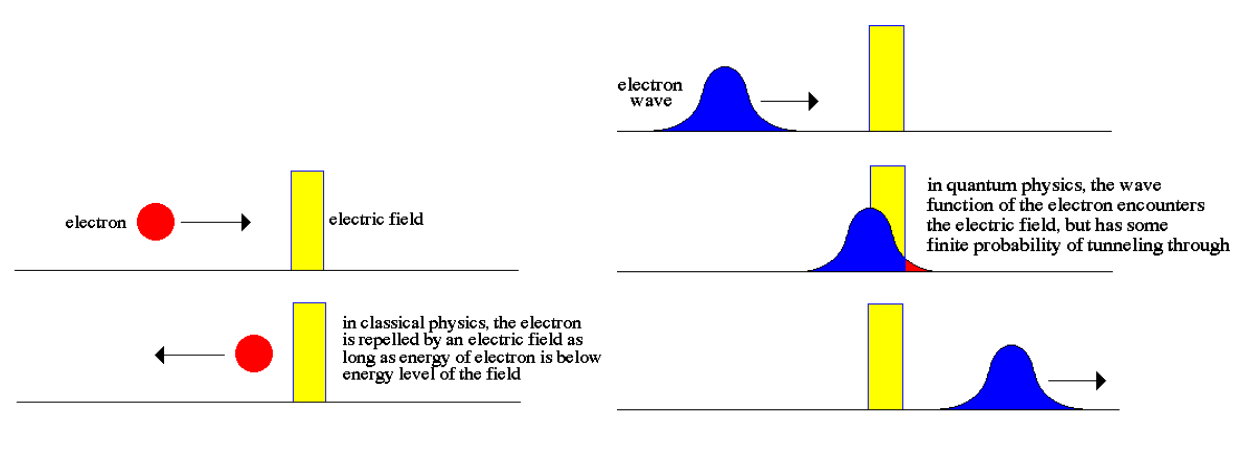
\includegraphics[width=0.5\textwidth]{TunnelingAll.png}
  \end{figure}

% Voor literatuurverwijzingen zijn er twee belangrijke commando's:
% \autocite{KEY} => (Auteur, jaartal) Gebruik dit als de naam van de auteur
%   geen onderdeel is van de zin.
% \textcite{KEY} => Auteur (jaartal)  Gebruik dit als de auteursnaam wel een
%   functie heeft in de zin (bv. ``Uit onderzoek door Doll & Hill (1954) bleek
%   ...'')

%---------- Methodologie ------------------------------------------------------
\section{Methodologie}
\label{sec:methodologie}

Om dit onderzoek te voltooien wordt er een algoritme gezocht die uitvoerbaar is op een klassieke computer.
Dit algoritme wordt dan omgezet naar een quantumalgoritme zodat het ook uitvoerbaar is op een quantumcomputer.
Dan worden er van beide de tijds- en ruimtecomplexiteit berekend. Om te bestuderen wat de effecten zijn van een verhoogd
aantal parameters wordt gezocht naar een algoritme die meer parameters kan accepteren. Dit wordt dan ook uitgevoerd op 
een kleine input (bv in een databank zoeken met een paar duizenden entries) en een grote input (enkele miljoenen entries).
Naast de vergelijking van het algoritme, wordt ook onderzocht naar het effect op de industie. Om dit te kunnen doen wordt er een
vragenlijst opgesteld die beantwoord moet worden door CEO's en CIO's van bedrijven. Uit de vragenlijst moet blijken wat
de belangrijkste bedrijfsprocessen zijn die verbeterd kunnen worden. Van deze processen wordt de complexiteit berekend en
worden deze dan vergeleken met het eerste algoritme. Op basis hiervan wordt dan een schatting gedaan wat het effect zal zijn
als dit proces uitgevoerd zou worden op een quantumcomputer. 

Het berekenen van de tijdscomplexiteit houdt niet veel meer in dan het tellen van het aantal elementaire stappen in het algoritme om dit ten einde te kunnen brengen.
Dit wordt beschreven in \textcite{Abhishek2021Tijd}. Er zijn 3 soorten complexiteit: constant, exponentieel (iets doen in 1 dimensie is lineair, in 2 dimensies kwadratisch enzoverder) of logaritmisch (het werk delen leidt tot een logoaritmische complexiteit).
Geheugen kan voor 3 dingen worden gebruikt: variabelen, de instructies en de executie van het algoritme. Zoals te lezen is in \textcite{Abhishek2021Ruimte} hangt de ruimtecomplexiteit voornamelijk af van het gebruikte geheugen in de executie van het algorimte.
Tijdens het uitvoeren wordt het geheugen op 3 verschillende manieren gebruikt: een deel gaat naar de instructies, een deel gaat naar de systeemstack waar alle variabelen van een algoritme op worden opgeslagen en wachten voor verdere uitvoer en als laatste gaat het geheugen ook naar  de data space (dit is het geheugen dat gebruikt wordt voor de variabelen en constanten).
Het meeste geheugen gaat naar de data space en daarom wordt meestal enkel dit gebruikt om de ruimtecomplexiteit te bereken. Ook in dit onderzoek zal dit zo gebeuren.
Om de ruimtecomplexiteit te bereken, moet er naar het datatype van de variabelen gekeken worden. Zo wordt een boolean bijvoorbeeld in 1 byte opgeslagen en een double in 8 bytes. 
Aan de hand van deze informatie kan de complexiteit gemakkelijk berekend worden.

Om het quantumalgoritme te schrijven en uit te voeren wordt er gebruik gemaakt van IBM's quantumcomputer. IBM heeft een online
tool om quantumalgortimes te maken en dan ook uit te voeren op hun computer.\footnote{\url{https://quantum-computing.ibm.com/}}

%---------- Verwachte resultaten ----------------------------------------------
\section{Verwachte resultaten}
\label{sec:verwachte_resultaten}

Voor de tijdscomplexiteit wordt er een verbetering verwacht die van de orde sqr(n) is.
Bij de ruimtecomplexteit wordt er geen verbetering verwacht aangezien er nog steeds evenveel geheugen nodig is om dezelfde processen uit te voeren.

Enkele van de verwachte voordelen zijn:
\begin{itemize} 
  \item Snellere rendering van complexe 3D-structuren zoals chemische componenten van pillen.
  \item Het sneller maken van meer efficiënte planningen die enkele of zelfs alle processen van een bedrijf voor een gegeven moment bepaald.
  \item Het doorzoeken van grote databanken kan sneller verlopen omdat een quantumcomputer dit in een sqr(n)-tijdsspanne kan doen.
  \item Simulaties van quantumfysica kunnen veel naukeuriger uitgevoerd worden.
  \item Machine learning verloopt veel efficiënter en kan dus voor betere AI-structuren zorgen.
  \item Het ontbinden van in priemfactoren van zeer grote getallen (dit kan de RSA-necryptie helemaal teniet doen).
\end{itemize}
%---------- Verwachte conclusies ----------------------------------------------
\section{Verwachte conclusies}
\label{sec:verwachte_conclusies}

Uit het onderzoek moet een vergelijking blijken tussen een klassieke computer en quantumcomputer. Met deze vergelijking moet er dan onderzocht worden of enkele belangrijke bedrijfsprocessen 
verbeterd kunnen worden door ze uit te voeren op een quantumcomputer. Naast de voordelen van dit zo te doen moet ook gebleken zijn wat de nadelen hiervan zijn.
Zo kan men later bij eventuele implemenaties van quantumcomputers al anticipiëren op de opgesomde nadelen en deze proberen te overbruggen.

%%---------- Andere bijlagen --------------------------------------------------
% TODO: Voeg hier eventuele andere bijlagen toe
%\input{...}

%%---------- Referentielijst --------------------------------------------------
\printbibliography[heading=bibintoc]

\end{document}
 